\documentclass[12pt]{article}

% Packages:
\usepackage{graphicx}
\usepackage[portuguese]{babel}
\usepackage[utf8]{inputenc}
\usepackage{setspace}
\usepackage{listings}
\usepackage{hyperref}
\usepackage{tocloft}
\usepackage{fancyhdr}
\usepackage{placeins}
\usepackage{subcaption}
\usepackage{subfiles}
\usepackage{outlines}
\usepackage{indentfirst}
\usepackage{amsmath}
\usepackage{enumerate}
\usepackage{subfiles}
\usepackage{color, colortbl, xcolor}
\usepackage{multicol}
%---

% Options:
\setstretch{1} % Espaçamento entre linhas
\usepackage[top=3cm, bottom=2cm, left=1.5cm, right=1.5cm]{geometry}
\PassOptionsToPackage{hyphens}{url}
\title{}
\date{}

% Code customization:
% Default fixed font does not support bold face
\DeclareFixedFont{\ttb}{T1}{txtt}{bx}{n}{10} % for bold
\DeclareFixedFont{\ttm}{T1}{txtt}{m}{n}{10}  % for normal

\lstset{
	basicstyle=\footnotesize,
	columns=fullflexible,
    keywordstyle=\ttb\color{blue},
	stringstyle=\ttm\color{green},
	commentstyle=\color{gray},
	frame=None,
	breaklines=true,
	showstringspaces=false,
	postbreak=\mbox{\textcolor{red}{$\hookrightarrow$}\space},
}

%---
% Document:
\begin{document}
	% Cabeçalho:
\begin{figure}
		\begin{minipage}{.3\linewidth}
			\centering
			\includegraphics[width=.6\linewidth]{imgs/ufpa.jpg}
		\end{minipage}
		\begin{minipage}{.70\linewidth}
			\flushleft
			\paragraph{}
			\textbf{ }\newline
			\textbf{UNIVERSIDADE FEDERAL DO PARÁ} \newline
			\textbf{INSTITUTO DE TECNOLOGIA} \newline
			\textbf{FACULDADE DE ENGENHARIA DA COMPUTAÇÃO E TELECOMUNICAÇÕES} \newline
			\textbf{TE05205 - Top. Especiais em Engenharia de Computação II} \newline
            \textbf{Prof. Dr. Roberto Celio Limão de Oliveira} \newline
            \textbf{Aluna: Camila Novaes Silva (201606840055)}
		\end{minipage}
\end{figure}
\FloatBarrier
\begin{center}
    {\Large \textbf{Exemplo de Otimização - Michalewicz 99}}
\end{center}
%%%%%%%%%%%%%
\hfill

O Algoritmo genético (AG) descrito a seguir foi implementado para solucionar um exemplo simples
de otimização, especificamente o de maximização de função de uma única variável. A função a ser
maximizada é $f(x) = x * sin(10\pi*x) + 1, x \in [-1..2]$.

Assim, o objetivo é encontrar o valor de $x$ dentro do intervalo $[-1..2]$ que maximiza a função
$f$, ou seja, encontrar $x_0$ tal que $f(x_0) \geq f(x) $ para todo $x \in [-1..2]$.

\begin{enumerate}[\textbf{(i)}]
	\item \textbf{Representação}
		\subitem Para representar todos os valores dentro do intervalo $[-1..2]$, com uma precisão
		de 6 casa decimais foram necessários 22 bits,
		$$2097152 = 2^{21} < 3*10^6 \leq 2^{22} = 4194304$$
		\subitem Para facilitar o trabalho de conversão entre números decimais e binário, podemos
		mapear as representações da seguinte forma:
			\subsubitem $0000000000000000000000_2 = d(0_{10}) = -1$
			\subsubitem $1111111111111111111111_2 = d(4194304_{10}) = 2$
		\subitem Logo, para fazer essa conversão utilizamos a seguinte formula:
		$$x_{real} = d(x') =  -1.0 + x' * \frac{3}{2^{22} - 1}$$
		\subitem Onde $x'$ é a conversão direta da base binária para a decimal.

	\item \textbf{Seleção}
		\subitem Algoritmo de seleção utilizado foi o torneio, com uma taxa de seleção de 0.25. E o fitness
		avaliado é igual ao valor de $f(x)$.
	\item \textbf{Operadores genéticos}
		\subitem Para realizar o cruzamento, foi utilizado o algoritmo ponto de corte. E a taxa de
		mutação foi de 1\%.
	\item \textbf{Critério de paragem}
		\subitem O critério de paragem foi 150 gerações.
\end{enumerate}

Os resultados obtidos são apresentados nas figuras abaixo.

\begin{figure*}[htb]
	\begin{center}
	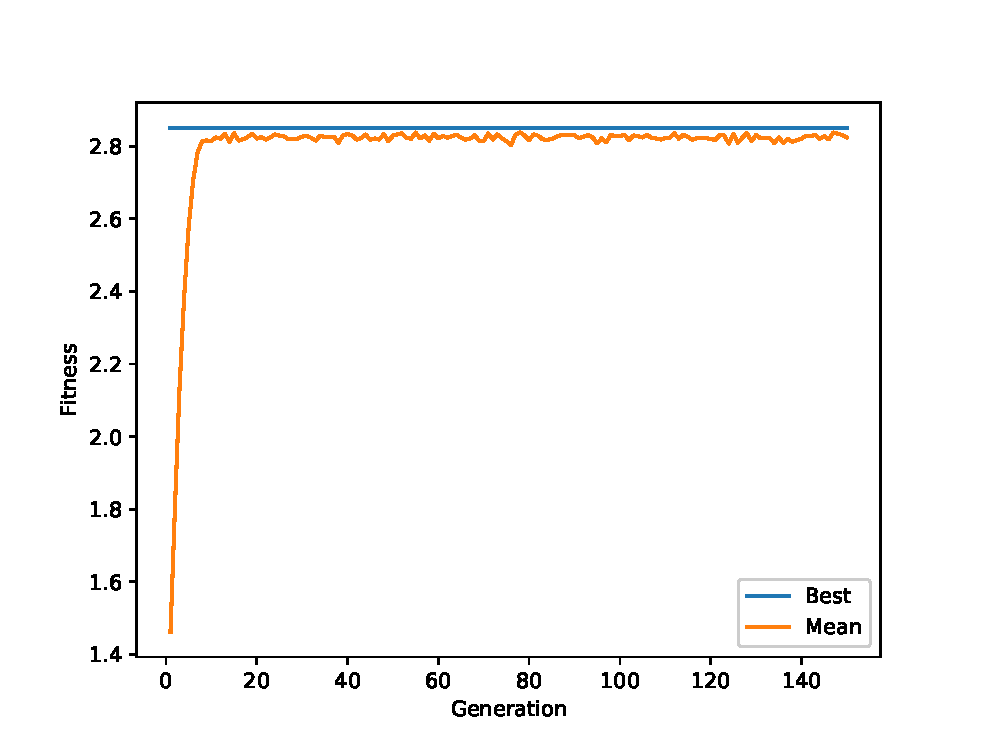
\includegraphics[width=0.5\textwidth]{./imgs/result-ag.eps}
	\caption{Resultado do AG.\label{fig:result}}
	\end{center}
\end{figure*}

\begin{figure*}[htb]
	\begin{center}
	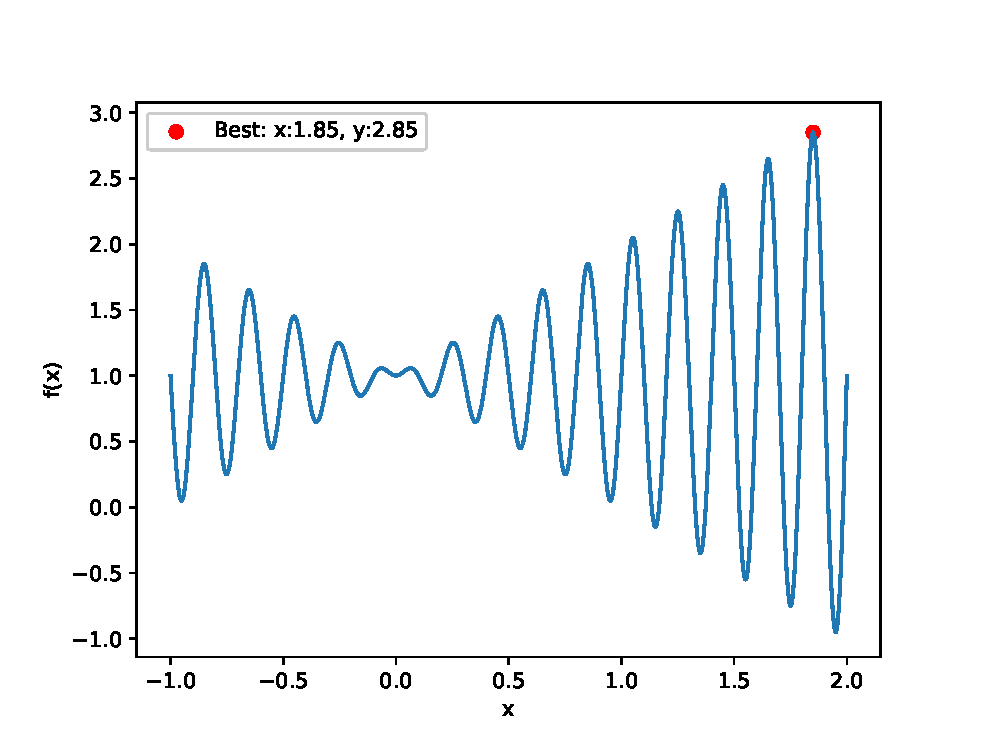
\includegraphics[width=0.5\textwidth]{./imgs/result2-ag.eps}
	\caption{Ponto máximo encontrado pelo AG na função $f(x)$.\label{fig:result}}
	\end{center}
\end{figure*}


\end{document}
